% answers.tex —— 2007 年·普通高等学校招生考试·福建卷·文科 · 参考答案与详细解析片段
% 由 tools/generate_projects.py 依来源总账自 2007/2007_数学真题_福建文_试题.md + 2007/2007_数学真题_福建文_解析正文.md + 2007/2007_数学真题_福建文_答案要点.md 生成，勿手改（改源 MD 后重跑）


\begin{gktip}
固定候选 PDF 仅含题面，无答案、解析和评分标准，原卷亦未标注分值；以下为非官方编者独立推导，官方答案字段为空。来源发布者、出版者、版次与官方身份均未核。
\end{gktip}

\begin{answer}
\gksolhead{1}{}

\textbf{题目}：

已知全集 $U=\{1,2,3,4,5\}$，且 $A=\{2,3,4\}$，$B=\{1,2\}$，则 $A\cap(\complement_UB)$ 等于（　）

（A）$\{2\}$

（B）$\{5\}$

（C）$\{3,4\}$

（D）$\{2,3,4,5\}$

\Needspace{4\baselineskip}
\textbf{解析}

\Needspace{5\baselineskip}
$\complement_UB=\{3,4,5\}$，故

\nopagebreak[4]
\[A\cap(\complement_UB)=\{2,3,4\}\cap\{3,4,5\}=\{3,4\}.\]

\gkanswer{答案：C。}

\end{answer}
\begin{answer}
\gksolhead{2}{}

\textbf{题目}：

等比数列 $\{a_n\}$ 中，$a_4=4$，则 $a_2\cdot a_6$ 等于（　）

（A）$4$

（B）$8$

（C）$16$

（D）$32$

\Needspace{4\baselineskip}
\textbf{解析}

\Needspace{5\baselineskip}
等比数列中 $a_2a_6=a_4^2$（下标 $2+6=4+4$），故

\nopagebreak[4]
\[a_2a_6=4^2=16.\]

\gkanswer{答案：C。}

\end{answer}
\begin{answer}
\gksolhead{3}{}

\textbf{题目}：

$\sin15^\circ\cos75^\circ+\cos15^\circ\sin105^\circ$ 等于（　）

（A）$0$

（B）$\dfrac12$

（C）$\dfrac{\sqrt3}2$

（D）$1$

\Needspace{4\baselineskip}
\textbf{解析}

\Needspace{5\baselineskip}
$\sin105^\circ=\sin75^\circ$，故

\nopagebreak[4]
\[\sin15^\circ\cos75^\circ+\cos15^\circ\sin105^\circ=\sin15^\circ\cos75^\circ+\cos15^\circ\sin75^\circ=\sin90^\circ=1.\]

\gkanswer{答案：D。}

\end{answer}
\begin{answer}
\gksolhead{4}{}

\textbf{题目}：

“$|x|<2$”是“$x^2-x-6<0$”的（　）

（A）充分而不必要条件

（B）必要而不充分条件

（C）充要条件

（D）既不充分也不必要条件

\Needspace{4\baselineskip}
\textbf{解析}

\Needspace{5\baselineskip}
$|x|<2$ 即 $-2<x<2$；由 $x^2-x-6<0$ 得

\nopagebreak[4]
\[-2<x<3.\]

$(-2,2)\subset(-2,3)$，故充分性成立；而 $x=\dfrac52$ 满足后者不满足前者，必要性不成立，所以是充分而不必要条件。

\gkanswer{答案：A。}

\end{answer}
\begin{answer}
\gksolhead{5}{}

\textbf{题目}：

函数 $f(x)=\sin\left(2x+\dfrac{\pi}3\right)$ 的图象（　）

（A）关于点 $\left(\dfrac{\pi}3,0\right)$ 对称

（B）关于直线 $x=\dfrac{\pi}4$ 对称

（C）关于点 $\left(\dfrac{\pi}4,0\right)$ 对称

（D）关于直线 $x=\dfrac{\pi}3$ 对称

\Needspace{4\baselineskip}
\textbf{解析}

\Needspace{5\baselineskip}
$f\left(\dfrac{\pi}3\right)=\sin\pi=0$，且对任意 $t$，

\nopagebreak[4]
\[f\left(\frac{\pi}3+t\right)+f\left(\frac{\pi}3-t\right)=\sin(\pi+2t)+\sin(\pi-2t)=-\sin2t+\sin2t=0,\]

故图象关于点 $\left(\dfrac{\pi}3,0\right)$ 对称。

其余选项：$f\left(\dfrac{\pi}4\right)=\sin\dfrac{5\pi}6=\dfrac12$，既不为 $0$ 也不为 $\pm1$，故关于 $x=\dfrac{\pi}4$、$\left(\dfrac{\pi}4,0\right)$ 的对称均不成立；同理 $x=\dfrac{\pi}3$ 处函数值为 $0$ 而非最值，关于直线 $x=\dfrac{\pi}3$ 也不对称。

\gkanswer{答案：A。}

\end{answer}
\begin{answer}
\gksolhead{6}{}

\textbf{题目}：

如图，在正方体 $ABCD-A_1B_1C_1D_1$ 中，$E$，$F$，$G$，$H$ 分别为 $AA_1$，$AB$，$BB_1$，$B_1C_1$ 的中点，则异面直线 $EF$ 与 $GH$ 所成的角等于（　）
\nopagebreak[4]
\begin{center}% 2007 年福建卷文科第 6 题：正方体 ABCD-A1B1C1D1，E、F、G、H 分别为
%   AA1、AB、BB1、B1C1 的中点，图中画出异面直线 EF 与 GH。
% 来源 PDF：gaokaomath-src/普通高考/2007/2007福建文.pdf
% SHA-256：96ffeae7fae0016108ed33e565abdf5983e06aef19f6452a8b4c8c5e5e4e58d0
% 原页：2007福建文.pdf 第 1 页（A3 三栏）第 1 栏，书页码 369。
% 重绘依据：按原页斜投影（前表面 ABB1A1、右表面 BCC1B1、上表面 A1B1C1D1）
%   与 A-D、D-C、D-D1 三条虚线重绘，E、F、G、H 均取棱的中点。
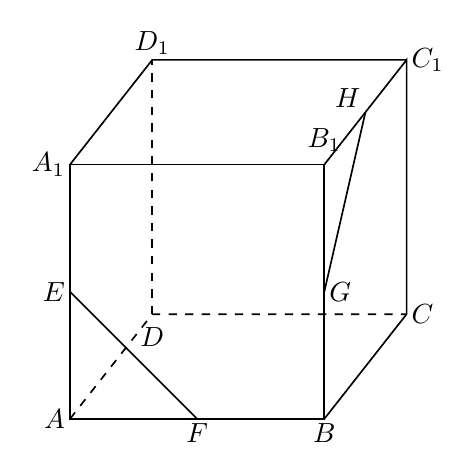
\begin{tikzpicture}[scale=0.95, semithick,
  every node/.style={inner sep=1.5pt}]

  \coordinate (A)  at (0.0,0.0);
  \coordinate (B)  at (3.4,0.0);
  \coordinate (C)  at (4.5,1.4);
  \coordinate (D)  at (1.1,1.4);
  \coordinate (A1) at (0.0,3.4);
  \coordinate (B1) at (3.4,3.4);
  \coordinate (C1) at (4.5,4.8);
  \coordinate (D1) at (1.1,4.8);
  \coordinate (E)  at (0.0,1.7);
  \coordinate (F)  at (1.7,0.0);
  \coordinate (G)  at (3.4,1.7);
  \coordinate (H)  at (3.95,4.1);

  % 可见的棱
  \draw (A) -- (B) -- (B1) -- (A1) -- cycle;
  \draw (B) -- (C) -- (C1) -- (B1);
  \draw (A1) -- (D1) -- (C1);

  % 被遮挡的棱
  \draw[dashed] (A) -- (D) -- (C);
  \draw[dashed] (D) -- (D1);

  % 异面直线 EF 与 GH
  \draw (E) -- (F);
  \draw (G) -- (H);

  \node[left] at (A) {$A$};
  \node[below] at (B) {$B$};
  \node[right] at (C) {$C$};
  \node[below=3pt] at (D) {$D$};
  \node[left] at (A1) {$A_1$};
  \node[above=3pt] at (B1) {$B_1$};
  \node[right] at (C1) {$C_1$};
  \node[above] at (D1) {$D_1$};
  \node[left] at (E) {$E$};
  \node[below] at (F) {$F$};
  \node[right] at (G) {$G$};
  \node[above left] at (H) {$H$};
\end{tikzpicture}
\end{center}
\nopagebreak[4]
（A）$45^\circ$

（B）$60^\circ$

（C）$90^\circ$

（D）$120^\circ$

\Needspace{4\baselineskip}
\textbf{解析}

\Needspace{5\baselineskip}
设正方体棱长为 $2$，取

\nopagebreak[4]
\[A(0,0,0),\ B(2,0,0),\ B_1(2,0,2),\ C_1(2,2,2),\ A_1(0,0,2),\]

\Needspace{5\baselineskip}
则各中点

\nopagebreak[4]
\[E(0,0,1),\quad F(1,0,0),\quad G(2,0,1),\quad H(2,1,2).\]

\Needspace{5\baselineskip}
于是

\nopagebreak[4]
\[\overrightarrow{EF}=(1,0,-1),\qquad \overrightarrow{GH}=(0,1,1),\]

\nopagebreak[4]
\[\cos\theta=\frac{\overrightarrow{EF}\cdot\overrightarrow{GH}}{\left|\overrightarrow{EF}\right|\left|\overrightarrow{GH}\right|}
=\frac{-1}{\sqrt2\cdot\sqrt2}=-\frac12.\]

异面直线所成的角取锐角，故为 $60^\circ$。

\gkanswer{答案：B。}

\end{answer}
\begin{answer}
\gksolhead{7}{}

\textbf{题目}：

已知 $f(x)$ 为 $\mathbf R$ 上的减函数，则满足 $f\left(\dfrac1x\right)>f(1)$ 的实数 $x$ 的取值范围是（　）

（A）$(-\infty,1)$

（B）$(1,+\infty)$

（C）$(-\infty,0)\cup(0,1)$

（D）$(-\infty,0)\cup(1,+\infty)$

\Needspace{4\baselineskip}
\textbf{解析}

\Needspace{5\baselineskip}
$f$ 在 $\mathbf R$ 上递减，故

\nopagebreak[4]
\[f\left(\frac1x\right)>f(1)\ \Longleftrightarrow\ \frac1x<1.\]

移项得 $\dfrac{1-x}x<0$，即 $x<0$ 或 $x>1$。

\gkanswer{答案：D。}

\end{answer}
\begin{answer}
\gksolhead{8}{}

\textbf{题目}：

对于向量 $\boldsymbol a$，$\boldsymbol b$，$\boldsymbol c$ 和实数 $\lambda$，下列命题中真命题的是（　）

（A）若 $\boldsymbol a\cdot\boldsymbol b=0$，则 $\boldsymbol a=\boldsymbol 0$ 或 $\boldsymbol b=\boldsymbol 0$

（B）若 $\lambda\boldsymbol a=\boldsymbol 0$，则 $\lambda=0$ 或 $\boldsymbol a=\boldsymbol 0$

（C）若 $\boldsymbol a^2=\boldsymbol b^2$，则 $\boldsymbol a=\boldsymbol b$ 或 $\boldsymbol a=-\boldsymbol b$

（D）若 $\boldsymbol a\cdot\boldsymbol b=\boldsymbol a\cdot\boldsymbol c$，则 $\boldsymbol b=\boldsymbol c$

\Needspace{4\baselineskip}
\textbf{解析}

（A）$\boldsymbol a\perp\boldsymbol b$ 时数量积为零而两向量均非零，假。

（B）$\lambda\boldsymbol a=\boldsymbol 0$ 时必有 $\lambda=0$ 或 $\boldsymbol a=\boldsymbol 0$，真。

（C）$\boldsymbol a^2=\boldsymbol b^2$ 只说明 $|\boldsymbol a|=|\boldsymbol b|$，方向可以不同，假。

（D）$\boldsymbol a\cdot\boldsymbol b=\boldsymbol a\cdot\boldsymbol c$ 只说明 $\boldsymbol a\perp(\boldsymbol b-\boldsymbol c)$，不能推出 $\boldsymbol b=\boldsymbol c$，假。

\gkanswer{答案：B。}

\end{answer}
\begin{answer}
\gksolhead{9}{}

\textbf{题目}：

已知 $m$，$n$ 为两条不同的直线，$\alpha$，$\beta$ 为两个不同的平面，则下列命题中正确的是（　）

（A）$m\subset\alpha$，$n\subset\alpha$，$m\parallel\beta$，$n\parallel\beta\Rightarrow\alpha\parallel\beta$

（B）$\alpha\parallel\beta$，$m\subset\alpha$，$n\subset\beta\Rightarrow m\parallel n$

（C）$m\perp\alpha$，$m\perp n\Rightarrow n\parallel\alpha$

（D）$n\parallel m$，$n\perp\alpha\Rightarrow m\perp\alpha$

\Needspace{4\baselineskip}
\textbf{解析}

（A）当 $m\parallel n$ 时两平面仍可相交，假。

（B）两平行平面内的直线可以异面，假。

（C）$m\perp\alpha$，$m\perp n$ 时 $n$ 可能落在 $\alpha$ 内，假。

（D）$n\perp\alpha$ 且 $m\parallel n$，则 $m$ 的方向也是 $\alpha$ 的法方向，故 $m\perp\alpha$，真。

【源疑点：原页（D）印作「$n\parallel m$，$n\subset\alpha\Rightarrow m\perp\alpha$」，其中 $n\subset\alpha$ 时结论不成立，四个选项便无一正确；按命题意图与四个选项的排布，此处应为 $n\perp\alpha$，本库照 $n\perp\alpha$ 转录并作答，特此说明。】

\gkanswer{答案：D。}

\end{answer}
\begin{answer}
\gksolhead{10}{}

\textbf{题目}：

以双曲线 $x^2-y^2=2$ 的右焦点为圆心，且与其右准线相切的圆的方程是（　）

（A）$x^2+y^2-4x-3=0$

（B）$x^2+y^2-4x+3=0$

（C）$x^2+y^2+4x-5=0$

（D）$x^2+y^2+4x+5=0$

\Needspace{4\baselineskip}
\textbf{解析}

双曲线 $x^2-y^2=2$ 中 $a^2=b^2=2$，$c=2$，右焦点 $F(2,0)$，右准线 $x=\dfrac{a^2}c=1$。

\Needspace{5\baselineskip}
圆以 $F$ 为圆心且与 $x=1$ 相切，半径 $r=2-1=1$，方程为

\nopagebreak[4]
\[(x-2)^2+y^2=1,\]

即 $x^2+y^2-4x+3=0$。

\gkanswer{答案：B。}

\end{answer}
\begin{answer}
\gksolhead{11}{}

\textbf{题目}：

已知对任意实数 $x$，有 $f(-x)=-f(x)$，$g(-x)=g(x)$，且 $x>0$ 时，$f'(x)>0$，$g'(x)>0$，则 $x<0$ 时，（　）

（A）$f'(x)>0$，$g'(x)>0$

（B）$f'(x)>0$，$g'(x)<0$

（C）$f'(x)<0$，$g'(x)>0$

（D）$f'(x)<0$，$g'(x)<0$

\Needspace{4\baselineskip}
\textbf{解析}

$f$ 为奇函数，其导函数为偶函数：$f'(-x)=f'(x)$，故 $x<0$ 时 $f'(x)=f'(-x)>0$。

$g$ 为偶函数，其导函数为奇函数：$g'(-x)=-g'(x)$，故 $x<0$ 时 $g'(x)=-g'(-x)<0$。

\gkanswer{答案：B。}

\end{answer}
\begin{answer}
\gksolhead{12}{}

\textbf{题目}：

某通讯公司推出一组手机号码，卡号的前七位数字固定，从“×××××××0000”到“×××××××9999”共 $10000$ 个号码。公司规定：凡卡号的后四位带有数字“$4$”或“$7$”的一律作为“优惠卡”，则这组号码中“优惠卡”的个数为（　）

（A）$2000$

（B）$4096$

（C）$5904$

（D）$8320$

\Needspace{4\baselineskip}
\textbf{解析}

后四位中不含 $4$、$7$ 的号码有 $8^4=4096$ 个，故含有 $4$ 或 $7$ 的号码有 $10000-4096=5904$ 个。

\gkanswer{答案：C。}

\end{answer}
\begin{answer}
\gksolhead{13}{}

\textbf{题目}：

$\left(x^2+\dfrac1x\right)^6$ 的展开式中常数项是\gkblank{}。（用数字作答）

\Needspace{4\baselineskip}
\textbf{解析}

\Needspace{5\baselineskip}
通项

\nopagebreak[4]
\[\mathrm C_6^k\left(x^2\right)^{6-k}\left(\frac1x\right)^k=\mathrm C_6^k x^{12-3k},\]

\Needspace{5\baselineskip}
常数项需 $12-3k=0$，即 $k=4$，系数为

\nopagebreak[4]
\[\mathrm C_6^4=15.\]

\gkanswer{答案：$15$。}

\end{answer}
\begin{answer}
\gksolhead{14}{}

\textbf{题目}：

已知实数 $x$，$y$ 满足 $\begin{cases}x+y\geqslant2,\\ x-y\leqslant2,\\ 0\leqslant y\leqslant3,\end{cases}$ 则 $z=2x-y$ 的取值范围是\gkblank{}。

\Needspace{4\baselineskip}
\textbf{解析}

\Needspace{5\baselineskip}
可行域顶点为 $(2,0)$、$(5,3)$、$(-1,3)$（分别为 $x+y=2$ 与 $y=0$、$x-y=2$ 与 $y=3$、$x+y=2$ 与 $y=3$ 的交点）。计算 $z=2x-y$：

\nopagebreak[4]
\[4,\qquad 7,\qquad -5,\]

故取值范围是 $[-5,7]$。

\gkanswer{答案：$[-5,7]$。}

\end{answer}
\begin{answer}
\gksolhead{15}{}

\textbf{题目}：

已知长方形 $ABCD$，$AB=4$，$BC=3$，则以 $A$，$B$ 为焦点，且过 $C$，$D$ 两点的椭圆的离心率为\gkblank{}。

\Needspace{4\baselineskip}
\textbf{解析}

\Needspace{5\baselineskip}
以 $A$，$B$ 为焦点，焦距 $2c=AB=4$，故 $c=2$。设 $A(0,0)$，$B(4,0)$，则 $C(4,3)$，且

\nopagebreak[4]
\[|CA|=\sqrt{4^2+3^2}=5,\qquad |CB|=3.\]

\Needspace{5\baselineskip}
椭圆过 $C$，故

\nopagebreak[4]
\[2a=|CA|+|CB|=8,\qquad a=4,\]

\Needspace{5\baselineskip}
离心率

\nopagebreak[4]
\[e=\frac ca=\frac12.\]

\gkanswer{答案：$\dfrac12$。}

\end{answer}
\begin{answer}
\gksolhead{16}{}

\textbf{题目}：

中学数学中存在许多关系，比如“相等关系”、“平行关系”等等。如果集合 $A$ 中元素之间的一个关系“$\sim$”满足以下三个条件：

① 自反性：对于任意 $a\in A$，都有 $a\sim a$；

② 对称性：对于 $a$，$b\in A$，若 $a\sim b$，则有 $b\sim a$；

③ 传递性：对于 $a$，$b$，$c\in A$，若 $a\sim b$，$b\sim c$，则有 $a\sim c$。

则称“$\sim$”是集合 $A$ 的一个等价关系。例如：“数的相等”是等价关系，而“直线的平行”不是等价关系（自反性不成立）。请你再列出两个等价关系：\gkblank{}。

\Needspace{4\baselineskip}
\textbf{解析}

三角形的相似关系满足自反性、对称性与传递性；整数的同余关系（同模 $n$ 的余数相同）同样满足三条性质。两例任写其一即可，答案不唯一。

\gkanswer{答案：例如：三角形的相似关系；整数的同余关系（模 $n$ 同余）。}

\end{answer}
\begin{answer}
\gksolhead{17}{}

\textbf{题目}：

在 $\triangle ABC$ 中，$\tan A=\dfrac14$，$\tan B=\dfrac35$。

（1）求角 $C$ 的大小；

（2）若 $AB$ 边的长为 $\sqrt{17}$，求 $BC$ 边的长。

\Needspace{4\baselineskip}
\textbf{解析}

\Needspace{5\baselineskip}
（1）由两角和的正切公式

\nopagebreak[4]
\[\tan(A+B)=\frac{\tan A+\tan B}{1-\tan A\tan B}
=\frac{\frac14+\frac35}{1-\frac14\cdot\frac35}
=\frac{\frac{17}{20}}{\frac{17}{20}}=1.\]

\Needspace{5\baselineskip}
$A$，$B$ 为三角形内角且正切为正，故 $A+B=45^\circ$，

\nopagebreak[4]
\[C=180^\circ-45^\circ=135^\circ.\]

\Needspace{5\baselineskip}
（2）由 $\tan A=\dfrac14$ 得 $\sin A=\dfrac1{\sqrt{17}}$。$AB=\sqrt{17}$ 为角 $C$ 的对边，由正弦定理

\nopagebreak[4]
\[\frac{BC}{\sin A}=\frac{AB}{\sin C},\]

\Needspace{5\baselineskip}
故

\nopagebreak[4]
\[BC=\sqrt{17}\cdot\frac{1/\sqrt{17}}{\sqrt2/2}=\sqrt2.\]

\gkanswer{答案：（1）$C=135^\circ$；（2）$BC=\sqrt2$。}

\end{answer}
\begin{answer}
\gksolhead{18}{}

\textbf{题目}：

甲、乙两名跳高运动员一次试跳 $2$ 米高度成功的概率分别为 $0.7$，$0.6$，且每次试跳成功与否相互之间没有影响，求：

（1）甲试跳三次，第三次才成功的概率；

（2）甲、乙两人在第一次试跳中至少有一人成功的概率；

（3）甲、乙各试跳两次，甲比乙的成功次数恰好多一次的概率。

\Needspace{4\baselineskip}
\textbf{解析}

记甲、乙一次试跳成功的概率 $p_1=0.7$，$p_2=0.6$，失败概率 $q_1=0.3$，$q_2=0.4$。

\Needspace{5\baselineskip}
（1）前两次失败、第三次成功：

\nopagebreak[4]
\[P=q_1^2p_1=0.3^2\times0.7=0.063.\]

\Needspace{5\baselineskip}
（2）至少一人成功，取对立事件“两人都失败”：

\nopagebreak[4]
\[P=1-q_1q_2=1-0.3\times0.4=0.88.\]

\Needspace{5\baselineskip}
（3）设甲、乙两次试跳的成功次数分别为 $X$，$Y$，则 $X\sim B(2,0.7)$，$Y\sim B(2,0.6)$，且相互独立。$X-Y=1$ 的情形为 $(X,Y)=(1,0)$ 与 $(2,1)$：

\nopagebreak[4]
\[P(X=1)=2\times0.7\times0.3=0.42,\qquad P(Y=0)=0.4^2=0.16,\]

\nopagebreak[4]
\[P(X=2)=0.7^2=0.49,\qquad P(Y=1)=2\times0.6\times0.4=0.48.\]

\Needspace{5\baselineskip}
故

\nopagebreak[4]
\[P=0.42\times0.16+0.49\times0.48=0.0672+0.2352=0.3024.\]

\gkanswer{答案：（1）$0.063$；（2）$0.88$；（3）$0.3024$。}

\end{answer}
\begin{answer}
\gksolhead{19}{}

\textbf{题目}：

如图，正三棱柱 $ABC-A_1B_1C_1$ 的所有棱长都为 $2$，$D$ 为 $CC_1$ 中点。

（1）求证：$AB_1\perp$ 平面 $A_1BD$；

（2）求二面角 $A-A_1D-B$ 的大小。
\nopagebreak[4]
\begin{center}% 2007 年福建卷文科第 19 题：正三棱柱 ABC-A1B1C1（底面正三角形、侧棱垂直底面，
%   所有棱长均为 2），D 为 CC1 的中点；图中画出 AB1、A1B、A1D、BD 等辅助线。
% 来源 PDF：gaokaomath-src/普通高考/2007/2007福建文.pdf
% SHA-256：96ffeae7fae0016108ed33e565abdf5983e06aef19f6452a8b4c8c5e5e4e58d0
% 原页：2007福建文.pdf 第 2 页（A3 三栏）第 1 栏，书页码 370。
% 重绘依据：按原页横放的三棱柱（左三角面 ABC、右三角面 A1B1C1）与虚线重绘；
%   C 为被遮挡的后顶点，A-C、B-C、C-C1 画虚线，D 取 CC1 中点。
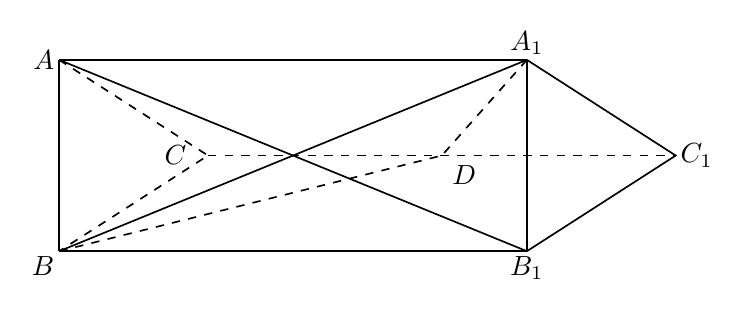
\begin{tikzpicture}[scale=0.9, semithick,
  every node/.style={inner sep=1.5pt}]

  \coordinate (A)  at (0.0,2.7);
  \coordinate (B)  at (0.0,0.0);
  \coordinate (C)  at (2.1,1.35);
  \coordinate (A1) at (6.6,2.7);
  \coordinate (B1) at (6.6,0.0);
  \coordinate (C1) at (8.7,1.35);
  \coordinate (D)  at (5.4,1.35);

  % 左三角面
  \draw (A) -- (B);
  \draw[dashed] (A) -- (C) -- (B);
  % 侧棱
  \draw (A) -- (A1);
  \draw (B) -- (B1);
  \draw[dashed] (C) -- (C1);
  % 右三角面
  \draw (A1) -- (B1);
  \draw (A1) -- (C1) -- (B1);
  % 题设辅助线
  \draw (A) -- (B1);
  \draw (A1) -- (B);
  \draw[dashed] (A1) -- (D);
  \draw[dashed] (B) -- (D);

  \node[left] at (A) {$A$};
  \node[below left] at (B) {$B$};
  \node[left=6pt] at (C) {$C$};
  \node[above] at (A1) {$A_1$};
  \node[below] at (B1) {$B_1$};
  \node[right] at (C1) {$C_1$};
  \node[below right=2pt] at (D) {$D$};
\end{tikzpicture}
\end{center}
\nopagebreak[4]
\Needspace{4\baselineskip}
\textbf{解析}

建立空间直角坐标系：取 $A(0,0,0)$，$B(2,0,0)$，$C(1,\sqrt3,0)$，$A_1(0,0,2)$，$B_1(2,0,2)$，$C_1(1,\sqrt3,2)$，则 $D$ 为 $CC_1$ 中点，$D(1,\sqrt3,1)$。

\Needspace{5\baselineskip}
（1）$\overrightarrow{AB_1}=(2,0,2)$。平面 $A_1BD$ 内两向量

\nopagebreak[4]
\[\overrightarrow{A_1B}=(2,0,-2),\qquad \overrightarrow{A_1D}=(1,\sqrt3,-1),\]

\Needspace{5\baselineskip}
其法向量

\nopagebreak[4]
\[\boldsymbol n=\overrightarrow{A_1B}\times\overrightarrow{A_1D}=\left(2\sqrt3,0,2\sqrt3\right)\parallel(1,0,1).\]

因 $\overrightarrow{AB_1}=2(1,0,1)\parallel\boldsymbol n$，故 $AB_1\perp$ 平面 $A_1BD$。

\Needspace{5\baselineskip}
（2）平面 $AA_1D$ 的法向量

\nopagebreak[4]
\[\boldsymbol n_1=\overrightarrow{AA_1}\times\overrightarrow{AD}=(0,0,2)\times(1,\sqrt3,1)=\left(-2\sqrt3,2,0\right)\parallel\left(-\sqrt3,1,0\right).\]

\Needspace{5\baselineskip}
平面 $A_1BD$ 的法向量可取 $\boldsymbol n_2=(1,0,1)$。两平面夹角 $\theta$ 满足

\nopagebreak[4]
\[\cos\theta=\frac{\left|\boldsymbol n_1\cdot\boldsymbol n_2\right|}{\left|\boldsymbol n_1\right|\left|\boldsymbol n_2\right|}
=\frac{\sqrt3}{2\sqrt2}=\frac{\sqrt6}4,\]

故二面角 $A-A_1D-B$ 的大小为 $\arccos\dfrac{\sqrt6}4$（约 $52.2^\circ$）。

【源疑点：原页第（2）问印作「二面角 $A-AD_1-B$」，但题设只定义了 $D$（$CC_1$ 中点），图中也没有 $D_1$，按图形与第（1）问的平面 $A_1BD$ 判断应为 $A-A_1D-B$，本库照此转录并作答。】

\gkanswer{答案：（1）证明见解析；（2）$\arccos\dfrac{\sqrt6}4$。}

\end{answer}
\begin{answer}
\gksolhead{20}{}

\textbf{题目}：

设函数 $f(x)=tx^2+2t^2x+t-1$（$x\in\mathbf R$，$t>0$）。

（1）求 $f(x)$ 的最小值 $h(t)$；

（2）若 $h(t)<-2t+m$ 对 $t\in(0,2)$ 恒成立，求实数 $m$ 的取值范围。

\Needspace{4\baselineskip}
\textbf{解析}

\Needspace{5\baselineskip}
（1）$t>0$，二次函数开口向上，对称轴

\nopagebreak[4]
\[x=-\frac{2t^2}{2t}=-t,\]

\Needspace{5\baselineskip}
故最小值

\nopagebreak[4]
\[h(t)=f(-t)=t\cdot t^2+2t^2\cdot(-t)+t-1=-t^3+t-1.\]

\Needspace{5\baselineskip}
（2）$h(t)<-2t+m$ 对 $t\in(0,2)$ 恒成立，等价于

\nopagebreak[4]
\[m>-t^3+3t-1\]

\Needspace{5\baselineskip}
对 $t\in(0,2)$ 恒成立。记 $g(t)=-t^3+3t-1$，则

\nopagebreak[4]
\[g'(t)=-3t^2+3=-3(t-1)(t+1).\]

\Needspace{5\baselineskip}
$0<t<1$ 时 $g'(t)>0$，$1<t<2$ 时 $g'(t)<0$，故 $g$ 在 $t=1$ 取最大值

\nopagebreak[4]
\[g(1)=1.\]

因此 $m>1$。

\gkanswer{答案：（1）$h(t)=-t^3+t-1$；（2）$m>1$。}

\end{answer}
\begin{answer}
\gksolhead{21}{}

\textbf{题目}：

数列 $\{a_n\}$ 的前 $n$ 项和为 $S_n$，$a_1=1$，$a_{n+1}=2S_n$（$n\in\mathbf N^*$）。

（1）求数列 $\{a_n\}$ 的通项 $a_n$；

（2）求数列 $\{na_n\}$ 的前 $n$ 项和 $T_n$。

\Needspace{4\baselineskip}
\textbf{解析}

\Needspace{5\baselineskip}
（1）由 $a_{n+1}=2S_n$：

\nopagebreak[4]
\[a_2=2S_1=2a_1=2.\]

\Needspace{5\baselineskip}
当 $n\geqslant2$ 时，$a_{n+1}=2S_n$ 与 $a_n=2S_{n-1}$ 相减得

\nopagebreak[4]
\[a_{n+1}-a_n=2a_n\ \Longrightarrow\ a_{n+1}=3a_n.\]

\Needspace{5\baselineskip}
故从 $a_2$ 起是公比 $3$ 的等比数列：

\nopagebreak[4]
\[a_1=1,\qquad a_n=2\cdot3^{n-2}\ (n\geqslant2).\]

\Needspace{5\baselineskip}
（2）$T_n=\sum\limits_{k=1}^n ka_k=1+2\sum\limits_{k=2}^n k\cdot3^{k-2}$。记

\nopagebreak[4]
\[S=\sum_{k=2}^n k3^{k-2}=\frac13\sum_{k=2}^n k3^{k-1}
=\frac13\left(\sum_{k=1}^n k3^{k-1}-1\right).\]

\Needspace{5\baselineskip}
利用 $\sum\limits_{k=1}^n kx^{k-1}=\dfrac{1-(n+1)x^n+nx^{n+1}}{(1-x)^2}$，取 $x=3$：

\nopagebreak[4]
\[\sum_{k=1}^n k3^{k-1}=\frac{1-(n+1)3^n+n3^{n+1}}4=\frac{1+(2n-1)3^n}4.\]

\Needspace{5\baselineskip}
于是

\nopagebreak[4]
\[S=\frac13\cdot\frac{(2n-1)3^n-3}4=\frac{(2n-1)3^n-3}{12},\]

\nopagebreak[4]
\[T_n=1+2S=1+\frac{(2n-1)3^n-3}6=\frac{(2n-1)3^n+3}6.\]

\gkanswer{答案：（1）$a_1=1$，$a_n=2\cdot3^{n-2}$（$n\geqslant2$）；（2）$T_n=\dfrac{(2n-1)3^n+3}6$。}

\end{answer}
\begin{answer}
\gksolhead{22}{}

\textbf{题目}：

如图，已知点 $F(1,0)$，直线 $l:x=-1$，$P$ 为平面上的动点，过 $P$ 作直线 $l$ 的垂线，垂足为点 $Q$，且 $\overrightarrow{QP}\cdot\overrightarrow{QF}=\overrightarrow{FP}\cdot\overrightarrow{FQ}$。

（1）求动点 $P$ 的轨迹 $C$ 的方程；

（2）过点 $F$ 的直线交轨迹 $C$ 于 $A$，$B$ 两点，交直线 $l$ 于点 $M$。

① 已知 $\overrightarrow{MA}=\lambda_1\overrightarrow{AF}$，$\overrightarrow{MB}=\lambda_2\overrightarrow{BF}$，求 $\lambda_1+\lambda_2$ 的值；

② 求 $\left|\overrightarrow{MA}\right|\cdot\left|\overrightarrow{MB}\right|$ 的最小值。
\nopagebreak[4]
\begin{center}% 2007 年福建卷文科第 22 题：定点 F(1,0)、直线 l:x=-1，P 为动点，Q 为 P 在 l 上的
%   垂足，且 QP·QF = FP·FQ；第（2）问过 F 的直线交轨迹 C 于 A、B，交 l 于 M。
% 来源 PDF：gaokaomath-src/普通高考/2007/2007福建文.pdf
% SHA-256：96ffeae7fae0016108ed33e565abdf5983e06aef19f6452a8b4c8c5e5e4e58d0
% 原页：2007福建文.pdf 第 2 页（A3 三栏）第 3 栏，书页码 370。
% 重绘依据：按原页只画坐标轴、准线 l 与焦点 F，并在 x 轴上标出 -1 与 1。
\begin{tikzpicture}[x=0.85cm, y=0.85cm, semithick,
  every node/.style={inner sep=1.5pt}]

  % 坐标轴
  \draw[->,>=stealth] (-3.2,0) -- (4.2,0) node[right] {$x$};
  \draw[->,>=stealth] (0,-2.4) -- (0,3.0) node[above] {$y$};
  \node[below left] at (0,0) {$O$};

  % 直线 l：x=-1
  \draw (-1,-2.0) -- (-1,2.6) node[above] {$l$};

  % 焦点 F
  \fill (1,0) circle (1.3pt);
  \node[above right=1pt] at (1,0) {$F$};

  % x 轴上的刻度 -1、1
  \node[below] at (-1,0) {$-1$};
  \node[below] at (1,0) {$1$};
\end{tikzpicture}
\end{center}
\nopagebreak[4]
\Needspace{4\baselineskip}
\textbf{解析}

\Needspace{5\baselineskip}
（1）设 $P(x,y)$，则 $Q(-1,y)$。于是

\nopagebreak[4]
\[\overrightarrow{QP}=(x+1,0),\qquad \overrightarrow{QF}=(2,-y),\]

\nopagebreak[4]
\[\overrightarrow{FP}=(x-1,y),\qquad \overrightarrow{FQ}=(-2,y).\]

\Needspace{5\baselineskip}
由 $\overrightarrow{QP}\cdot\overrightarrow{QF}=\overrightarrow{FP}\cdot\overrightarrow{FQ}$：

\nopagebreak[4]
\[2(x+1)=-2(x-1)+y^2,\]

\Needspace{5\baselineskip}
化简得

\nopagebreak[4]
\[y^2=4x.\]

\Needspace{5\baselineskip}
（2）① 设过 $F(1,0)$ 的直线为 $y=k(x-1)$（$k\neq0$），与 $l:x=-1$ 交于

\nopagebreak[4]
\[M(-1,-2k).\]

\Needspace{5\baselineskip}
代入 $y^2=4x$：

\nopagebreak[4]
\[k^2(x-1)^2=4x\ \Longrightarrow\ k^2x^2-(2k^2+4)x+k^2=0.\]

\Needspace{5\baselineskip}
设 $A(x_1,y_1)$，$B(x_2,y_2)$，则

\nopagebreak[4]
\[x_1+x_2=2+\frac4{k^2},\qquad x_1x_2=1.\]

\Needspace{5\baselineskip}
由 $\overrightarrow{MA}=\lambda_1\overrightarrow{AF}$ 比较横坐标：$x_1+1=\lambda_1(1-x_1)$，故

\nopagebreak[4]
\[\lambda_1=\frac{x_1+1}{1-x_1};\]

\Needspace{5\baselineskip}
同理 $\lambda_2=\dfrac{x_2+1}{1-x_2}$。于是

\nopagebreak[4]
\[\lambda_1+\lambda_2=\frac{(x_1+1)(1-x_2)+(x_2+1)(1-x_1)}{(1-x_1)(1-x_2)}
=\frac{2-2x_1x_2}{1-(x_1+x_2)+x_1x_2}.\]

\Needspace{5\baselineskip}
代入 $x_1x_2=1$ 得分子为 $0$、分母为 $1-(x_1+x_2)+1\neq0$，故

\nopagebreak[4]
\[\lambda_1+\lambda_2=0.\]

\Needspace{5\baselineskip}
②

\nopagebreak[4]
\[\left|\overrightarrow{MA}\right|=\sqrt{1+k^2}\left|x_1+1\right|,\qquad
\left|\overrightarrow{MB}\right|=\sqrt{1+k^2}\left|x_2+1\right|,\]

\Needspace{5\baselineskip}
故

\nopagebreak[4]
\[\left|\overrightarrow{MA}\right|\left|\overrightarrow{MB}\right|=(1+k^2)\left|x_1x_2+x_1+x_2+1\right|
=(1+k^2)\left(2+2+\frac4{k^2}\right)
=4\left(2+k^2+\frac1{k^2}\right).\]

\Needspace{5\baselineskip}
由均值不等式 $k^2+\dfrac1{k^2}\geqslant2$，等号在 $k^2=1$ 时成立，故最小值为

\nopagebreak[4]
\[4(2+2)=16.\]

\gkanswer{答案：（1）$y^2=4x$；（2）① $0$；② $16$。}

\end{answer}